
\documentclass[10pt, conference, compsocconf]{IEEEtran}
\usepackage{graphicx}


% correct bad hyphenation here
\hyphenation{op-tical net-works semi-conduc-tor}
\usepackage{cite}

\begin{document}
%
% paper title
% can use linebreaks \\ within to get better formatting as desired
\title{A fuzzy logic approach to \\collision avoidance in smart UAVs \\ Technical Report \#CSSE12-05 \\}


% author names and affiliations
% use a multiple column layout for up to two different
% affiliations

\author{
\IEEEauthorblockN{Michelle Hromatka}
\IEEEauthorblockA{Computer Science Dept.\\
College of Saint Benedict \textbar \hspace{1pt} Saint John's University\\
St. Joseph, MN\\
mthromatka@csbsju.edu}
\\
\\
\IEEEauthorblockN{Matt Holt}
\IEEEauthorblockA{Computer Science Dept.\\
Auburn University\\
Auburn, AL\\
holtjma@tigermail.auburn.edu}
\and
\IEEEauthorblockN{Jeffrey West}
\IEEEauthorblockA{Mechanical Engineering Dept.\\
University of Southern California\\
Los Angeles, California\\
jeffrey.west@usc.edu}
\\
\\
\IEEEauthorblockN{Saad Biaz}
\IEEEauthorblockA{Computer Science Dept.\\
Auburn University\\
Auburn, AL\\
biazsaa@auburn.email.edu}
}

% make the title area
\maketitle

\begin{abstract}
In recent years there has been an increase of interest related to collision avoidance techniques for unmanned aerial vehicles. Many approaches have been proposed but very few have been tested in high density, fixed speed test conditions. Our approach uses fuzzy logic to determine an appropriate avoidance maneuver after a possible collision is detected. Initially fuzzy logic was also used to detect possible collisions, the reasons this level was removed from the final results are detailed within.  This method was chosen for its adaptability, ease of implementation, and robustness with inadequate sensing techniques. This approach is explained in detail and the simulated results are presented after testing on two different field sizes, each with four levels of plane density. 
\end{abstract}

\begin{IEEEkeywords}
UAV; collision avoidance; fuzzy logic;9

\end{IEEEkeywords}





\section{Introduction}
Collision avoidance techniques for unmanned aerial vehicles have been a popular area of study in the field of intelligent robotics. In order for these vehicles to be used in areas such as surveillance or exploration, the vehicles must be able to autonomously react to static or dynamic obstacles while maintaining an efficient path.  Many approaches have been taken, including path planning, potential fields,  geometric and fuzzy logic methods. We first outline the problem in section two, then move on to describe the various approaches to solving the problem, including our chosen approach of using fuzzy logic to avoid detected collisions.
\section{Problem Statement}
Many algorithms exist to solve the general problem of UAV collision avoidance, but few of these algorithms have been tested in similar test conditions. In order to synthesize results and compare many algorithms in a single simulation, Holt et al. developed a simulator for comparison of various algorithms \cite{holtthesis}.  By using the simulator, different algorithms can be tested using the same metrics and flight constraints on the same platform. All algorithms are tested in two dimensions, with UAVs traveling at a constant speed of 25 miles per hour. Turning radius was modeled after an EasyStar RC aircraft and limited to 22.5 degrees per second. Telemetry updates are retrieved once per second, and new waypoints directing the UAV can be sent once per second. Environmental factors are also excluded from simulation.

The simulator was designed to test algorithms for real-time calculations. Regardless of how long calculations take, the simulator runs in real-time and new telemetry updates will be generated once per second. If no new waypoints are generated from the calculations in time, the current heading will be followed until a waypoint is received.

Two metrics were chosen to determine effectiveness.  A {\it near miss} is defined as one UAV traveling within a radius of 12 meters of another UAV. This is meant to represent a collision, as 12 meters represents approximately the distance travelled in one timestep, and should be avoided at all costs. Similarly, a {\it conflict} is defined as one UAV traveling within a radius of 24 meters of another UAV, or approximately two timesteps. This represents the danger zone and should be avoided, but is not as critical as a near miss. Both are shown in Figure \ref{fig:nearMissAndConflict}.

\begin{figure}[position here]
\centering
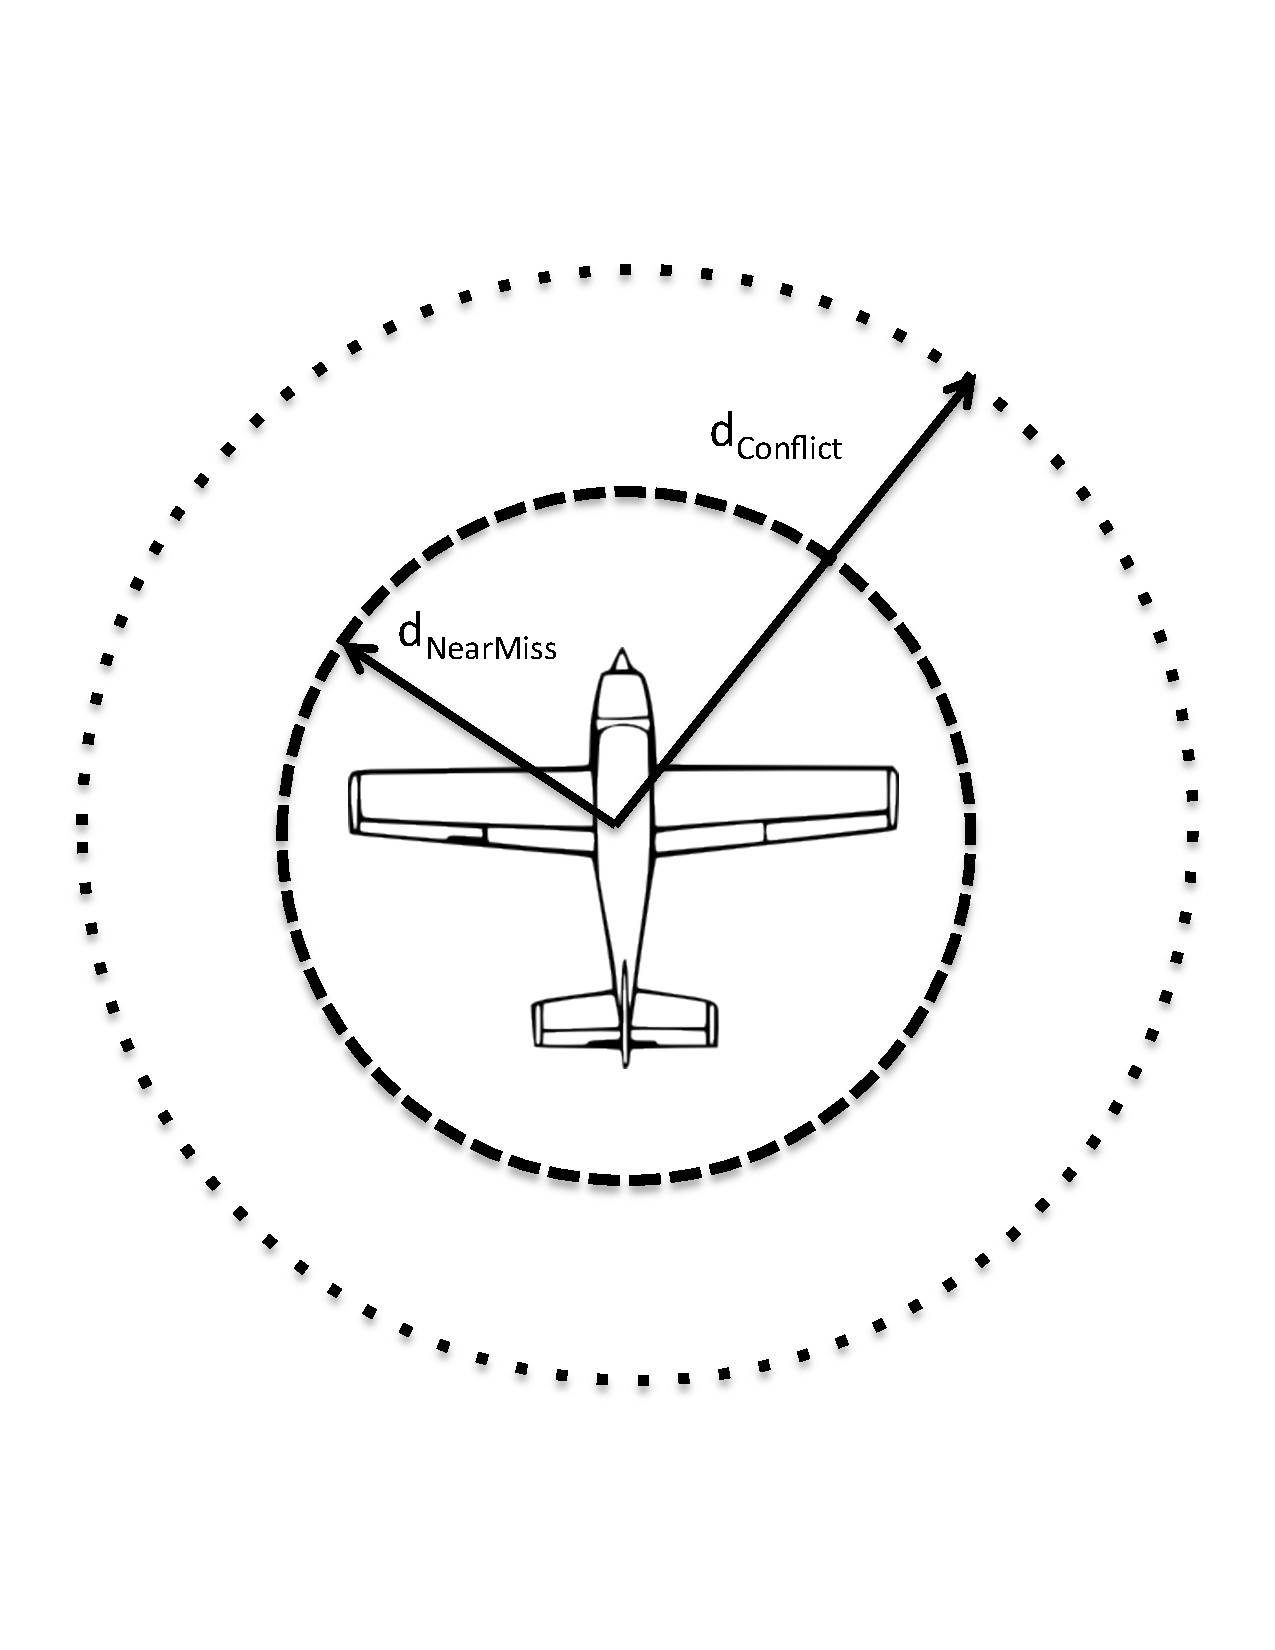
\includegraphics[scale=0.25]{EPS/nearMiss}
\caption{Near Miss and Conflict}
\label{fig:nearMissAndConflict}
\end{figure}

A separate metric was chosen to provide a measure of effectiveness. This is determined by the number of goal positions, or waypoints that a UAV achieves. An overly cautious algorithm may avoid near misses or conflicts very well, but the overall number of waypoints reached will be decreased. A delicate balance of effectiveness and efficiency for each algorithm must be achieved. The simulation time limit is ten minutes, and based on the number of near misses and waypoints reached, an algorithm's effectiveness can be measured. Note: for the purposes of this paper, parameters were optimized for low collisions (high effectiveness). As with any algorithm, parameters can be adjusted for better efficiency if some collisions are an acceptable sacrifice for better efficiency.

Previous research has tested Mixed Integer Linear Programing (MILP), Dynamic Sparse A* Algorithm, and Artificial Potential Fields in this simulation \cite{holtthesis}.  Each algorithm was run in eight different field situations: a 500m square field and a 1000m square field, each tested with 4, 8, 16 and 32 planes.  This will allow for easy comparison of methods presented here to those previously tested.
 
\section{Literature Review}
The literature review is split into the following sections: path planning, potential fields, proportional navigation, fuzzy logic, and hybrid approaches. Within these sections, the previously tested Mixed Integer Linear Programming (MILP), Artificial Potential Fields (APF), A* Grid Based Algorithm will be  reviewed and explored for strengths and weaknesses.  As mentioned in \cite{holtthesis},  the general goal of this research is to compare various algorithms using the same simulation and metrics, as outlined above. The next section will provide a comprehensive literature review of fuzzy logic as it has been used in collision avoidance.  The justification of this approach will be outlined in the methods section.

\subsection{Path Planning}
Path planning methods have also been researched using different techniques for finding an optimal path such as Mixed Integer Linear Programming (MILP) and A* search.  This approach tries to plan a collision free path for each plane in the field space. There are some other path planning techniques, but these are mainly used to increase efficiency in the chosen path, not for finding a collision-free path.

\subsubsection{MILP}
\cite{schouwenaars2001mixed} successfully used MILP for a solution to single and multi-vehicle path planning algorithm with both static and moving obstacles.  One of the major advantages of MILP solvers is the ability to limit inputs and outputs; this is useful in UAV collsion avoidance where the maximum turning radius is clearly defined.  A receding horizon is a common implementation of the MILP approach. This strategy limits the solution to a specified number of time steps into the future, as opposed to solving the entire system, thus an optimal path is found multiple times. A fixed arrival time approach finds an optimal path once but for the entire field. This method is often limited by heavy computational load; the solver is not guaranteed to come up with a solution, especially for many UAVs in a relatively small space, before collisions occur \cite{schouwenaars2001mixed}.  For this reason the receding horizon approach is widely used, but still not infallible.  A horizon time limit should not be so short that the vehicles will not have sufficient time to react and avoid collisions, nor should the time be so long that heavy computational load is still an issue. There are some optimization techniques that have been used to counter the issues that come with truncating the horizon time \cite{mettler2008receding}.  According to the simulation from Holt et. al., MILP was tested using a licensed online MILP solver in high density testing conditions. The receding horizon approach and other optimization techniques were used, however, the system still failed for more than 8 vehicles in a 500m square airspace \cite{lastyearMILP}.  The optimization techniques used were solver time limit, specifying the max amount of time before reverting to a sub-optimal solution, and the use of a "loiter cycle" which the UAV enters until the solver can come up with a solution.  The latter solution is not ideal when evaluating an algorithm's efficiency.

\subsubsection{A* Search Algorithm}
Another path planning algorithm is that of A* search, or the {\it branch and bound} method.  In this technique, the field space is divided into a grid and only adjacent squares are considered as a next point along the path.  This consideration of other nodes is called {\it branching}, estimating the best path from the current square is known as {\it bounding}.  When a square is branched, the cost is computed based off of a heuristic cost function. Each square with its corresponding cost is inserted into a tree structure, typically a heap, which stores the minimum element as the root. As the heap is updated from node to node, the lowest cost path is always at the top of the heap.  If the path that the algorithm is considering is no longer the lowest cost, a lower cost option is readily available, and that path is followed until either a lower cost path is found or the goal point is reached \cite{lastyearDSAS}.  One of the major issues with the A* search approach is determining an appropriate cost function.  As with other path planning techniques, computation time is an issue for real-time collision avoidance. There are some ways to lower computation time, especially if the optimum solution is not required but a nearly optimal path is acceptable. 

Other literature has used the A* search to determine the best path for a humanoid robot to place its footsteps in an obstacle littered space \cite{kuffner2005motion}.  In this case, the foot placement options were limited to 15 locations from each previous footstep.

\begin{figure}[position here]
  \centering
    \includegraphics[width=0.5\textwidth]{EPS/AStarRobot}
  \caption{The degrees of freedom allowed for the humanoid robot's right foot \cite{kuffner2005motion}}
\end{figure}

For their path, specified at 18 footsteps, the unconstrained A* search tree would contain approximately $10^{21}$ nodes. By limiting the options that A* considers, the final tree contained around 830,000 nodes, significantly less than the predicted $10^{21}$ nodes. By limiting the degrees of freedom allowed in the bounding step, the computation time is decreased dramatically, however, this approach is still too compuationally demanding for high density systems. As seen in \cite{liao2012uav} and \cite{lastyearDSAS}, this algorthm was tested in situations of varying plane density using the maximum turning radius as a limitation on the degrees of freedom allowed.  In each of these cases, A* performed well for low density airspaces, but still yielded many near-misses for dense systems.  

\subsection{Potential Fields}
\subsubsection{Artificial Potential Fields}
The potential field path planning approach can be split into two different categories: global and local.  The global solution requires a priori knowledge of the field and location of the obstacles within that field. Negative charges are applied to the obstacles and the goal point is assigned a positive charge. The robot is then driven to the goal point by the forces equal to the negative gradient of the field \cite{park2001obstacle}. 

\begin{figure}[position here]
  \centering
   \includegraphics[width=0.5\textwidth]{EPS/potentialFieldPathPlanning}
  \caption{The gradient along which the UAV is directed \cite{potFieldPic}.}
\end{figure}

Similar to other global path planning algorithms, global potential field path planning has very high computation costs, especially with robots that have many degrees of freedom, which makes it unsuitable for real-time path planning.  The local potential field approach is much more suitable in real-time solution planning.  Real-time, local solutions allow for both static and dynamic obstacles, making solutions much more reactive and realistic. The local potential field approach is set up similarly to the global approach, the path for the robot determined by the sum of forces acting on the robot \cite{hwang1992potential}. Potential field path planning methods are computationally efficient for finding a local obstacle-free path, however this method is not without its faults. As \cite{park2001obstacle} clearly asserts, there is a well-documented problem with the potential field approach: local minima.  When a robot experiences equal and opposite forces acting upon it, the robot can become stuck in a local minimum.  In purely dynamic obstacle avoidance environments, the local minimum problem is likely to have resolved itself by the next timestep, however the interval between timesteps might be enough that a possible collision becomes unavoidable. 

%10.1.1.57.9509
\subsubsection{Total Field}
Several implementations of UAV collision avoidance using real world applications have also been used in addition to simulation studies. One approach uses magnetic fields and magnetic sensors to detect nearby UAVs \cite{sigurd2003uav}. The goal of this approach is to have decentralized collision avoidance. A gradient is computed based on objects sensed, and the UAV will be directed to travel in opposition to the gradient. Field size decreases by the inverse of distance cubed. The results were found through simulation, but some real world magnetic sensor readings and reaction tests were conducted to see if the movements seen in the simulator were realistic. These methods worked well for collision avoidance, but yielded sub optimal paths. 

For the purposes of this paper, any algorithms are tested in simulation, but the research goal of developing a decentralized method of collision avoidance is seen as advantageous.  As Sigurd states, the problem of collision avoidance rapidly becomes intractable using centralized methods as the number of vehicles increases, making a decentralized approach where each vehicle is responsible for its own trajectory planning desirable \cite{sigurd2003uav}.

\subsection{Proportional Navigation}
Through the course of literature review, several other types or variations of algorithms were considered. One such algorithm, Proportional Navigation-Based Optimal Collision Avoidance Guidance for UAVs is widely used in missile guidance problems, and it can be used in collision avoidance by guiding the relative velocity vector to the collision avoidance vector \cite{han2004proportional}. The research proposed a collision avoidance law based on conventional Proportional Navigation (PN) guidance law. First, a collision avoidance vector is defined and the heading of the aircraft is directed toward this vector. The total approach is called Proportional Navigation-based Collision Avoid Guidance (PNCAG). The approach uses the collision cone geometric method  to determine when to enter the collision avoidance mode \cite{chakravarthy1998obstacle}. Several conditions for collision avoidance must be met including a range between aircraft and obstacle greater than safety distance, the direction of relative velocity must be outside of the collision cone, and the obstacle must be located behind the direction of the relative velocity vector. These techniques have shown promising results in both efficiency and effectiveness.

\subsection{Fuzzy Logic}
A common technique used in ground robot collision avoidance is that of fuzzy logic.  Fuzzy logic is a form of many valued logic which instead of outputting a 0 or 1, true or false value, instead outputs a degree of truth.  Fuzzy membership sets will map the crisp value to a fuzzy value.  For example, if height:short is defined as 50 - 70 inches, and height:tall is defined as  65 - 85 inches, a person could belong to both sets height:short and height:tall because fuzzy logic allows values to be a member of two sets at once \cite{fuzzyBook}. This is a more intuitive form of logic and a better represenation of the way humans think. A person is not always exclusively short or exclusively tall, rather someone is "kind of tall". Similarly, fuzzy logic can be applied to collision avoidance with output membership sets such as "very left" or "slightly right."Using a fuzzy logic system also allows for sensor fusion, when data from multiple sensors are combined. 

For these reasons, fuzzy logic research is frequently used and shown to work in mobile ground robots where sensing techniques are generally inexpensive and inaccurate. Sensor fusion has been accomplished using fuzzy logic in a sense-act approach based on multiple sensors distributed around a 2-D ground robot \cite{martinez1993fuzzy}.This approach was used in situations containing only one robot and stationary obstacles.  The mobile ground robot was run through a path containing obstacles where the smoothness of the path was evaluated. Advantages of the fuzzy logic approach are intuitive linguistic terms and a smaller computational load than APF and many other approaches. Fuzzy logic is also useful for unknown and semi-unstructured environments. Sense-act is uninterrupted motion with short development time and incorporates flexibility, easy to adjust parameters. 

\subsection{Hybrid Approach}
1) Fuzzy Logic / Electrostatic Potential Fields \\
Many approaches to UAV collision avoidance use a combination of two or more methods. An example of one of these hybrid approaches used fuzzy logic to control an autonomous mobile robot(AMR) while travelling along a pre-planned path generated by a total field path planning technique. A 2-layer fuzzy logic (FL) interface was combined with an electrostatic potential field path planner (EPF) to provide real-time mobile robot navigation in a 2-D dynamic environment \cite{tsourveloudis2001autonomous}. The first layer of fuzzy logic provided a sensor fusion system to combine data from several sonar sensors returning two fuzzy variables, direction and distance in four directions:front, back, left, and right. The second layer provided an obstacle detection module that outputs the position and degree of possibility which a collision may occur. This information is combined in motion control module with the path planner output.  If an obstacle blocks the pre-planned EPF path, collision avoidance maneuvers affecting heading and speed are used to avoid the detected collision.

This EPF/FL approach combined planned and reactive behavior into one algorithm.  EPF path planning reacts slowly to unknown moving obstacles. The EPF/FL approach allowed EPF to plan the path and allowed the fuzzy inference system to implement the path while avoiding collisions with all obstacles. Some discussion was given into tuning the membership functions, however, no analytical method guarantees optimal selection for the Mamdani-type FL inference systems. Several approaches have been used to tune membership functions, such as neural nets, genetic algorithms, and neuro-fuzzy methods, but none of these approaches guarantee as optimal solution \cite{tsourveloudis2001autonomous}.  Additionally, advantages of EPF compare to other potential field solutions were concluded. Collision free paths generated by the EPF method necessarily lead the UAV toward the goal, local minima are not generated within the field and stagnation points within the field do not exist. The path planned by EPF also generates an optimal minimum occupancy path toward the goal \cite{tsourveloudis2001autonomous}.

There are several limitations when applying much of this research to UAV collision avoidance . First, many of the obstacles in this research are static, which is not directly applicable to UAV collision avoidance with multiple UAVs. Mobile ground robots have fewer limitations of freedom of motion than do UAVs. Changes in speed, reversing direction and a $360^\circ$ turning radius are components of many 2-D ground robots, all three of which are not allowed or limited in this UAV collision avoidance research. 

One example of using fuzzy logic in UAV collision avoidance was found. In this scenario, a pre-planned path for the UAV was used until a collision was detected.  The obstacles were of varying shape and size and the avoidance technique sensed these two factors, then found an avoidance maneuver that deviated from the pre-planned path. Again, obstacles were static and changes in speed were allowed in determining an appropriate avoidance maneuver.  The UAV was able to successfully avoid collisions with one or multiple obstacles in all cases presented \cite{dong2005path}. More information on this approach is detailed in the Methods section, as we use this as the basis for the formation of our fuzzy logic collision avoidance system. 

2) Path Planning / Reactive Avoidance \\
Another hybrid approach used a hybrid of path planning and reactive collision avoidance \cite{manathara2011reactive}. This algorithm calculated a Dubins path for each plane then considered only the most imminent predicted collision for each aircraft. The line of sight (LOS) rate between the two planes is then increased. When a UAV detects multiple planes that are on a collision course with itself, it will select the most imminent collision to avoid that has a predicted zero effort miss (ZEM) of less than the minimum desired separation. The LOS is increased by applying a lateral acceleration to increase the rate of rotation of the LOS connecting these two UAVs. The UAV takes the sharpest turn available until the collision course is avoided.

This research uses very different simulation and metrics to test this algorithm. Planes initial positions are chosen to be evenly spaced around a circle that dictates the outside of the test space. A random goal point is published for each plane, somewhere on a smaller concentric circle. This setup eliminates the chance that random plane positions will be chosen in the test space that are actually {\it inside} or very near to a conflict zone of another plane. The PNCAG's simulation setup, however, does not take into account multiple waypoints. Efficiency of the algorithm was measured by deviation from initial Dubins path. 

PNCAG was found to be very efficient as well as effective in reducing the number of near-misses. With an outer circle radius of 500 meters, 20 to 60 UAVs were simulated, giving comparable scenarios to current research goals. The efficiencies achieved were very good (around 90 percent or higher), however, the research cannot be completely compared to results here because multiple waypoints were not achieved (the values were averaged over 10 runs with a single waypoint goal here) and the simulation starting points and goals were chosen in an advantageous manner, as described before.

3) Passive Pre-Planning / Geometric Reactive \\
Another hybrid approach used a passive approach to collision detection and avoidance \cite{angelov2008passive}. The research split the collision avoidance process into three steps, all defined by two plane's relative bearing angle: detection, avoidance, and an optimal return to pre-planned path. After calculating the bearings between the two planes that are at risk of colliding, a geometric approach is used to determine the necessary turning angle necessary to avoid a collision. The minimum separation distance between two UAVs can also be specified. Results of this method were promising, but only two scenarios, overtaking and front collision were presented in this research. This research is more applicable as an addition to algorithms that may have limited effectiveness in these two special cases.

\section{Methods}
Methods here build upon research described previously: work done by Dong et al. and Tsourveloudis.  The two-tiered fuzzy logic system used in Tsourveloudis \cite{tsourveloudis2001autonomous} was combined here with the fuzzy logic collision avoidance used by Dong \cite{dong2005path} to develop an efficient and effective algorithm that could handle high-density flight situations. 

\subsection{Collision Detection System}
Similar to Tsourdeveloudis' multi level fuzzy system, the first level fuzzy logic controller served as a method to detect possible collisions.  Considering only the closest UAV, the first tier used fuzzy logic to output a danger value denoting the likelihood of a collision between the current UAV and the closest UAV. The danger value was determined by inputs of {\it distance to collision}, ($d_{col}$), and {\it overlap distance}, ($d_{ovlp}$). Both variables are defined below and a graphical representation of these two inputs can be seen in Figure \ref{fig:basicPic}.

\begin{equation}
d_{col} = min(d_{A}, d_{B})
\end{equation}
\begin{equation}
d_{ovlp} = d_{A} - d_{B}
\end{equation}

\begin{figure}[h]
\centering
\includegraphics[scale=0.3]{EPS/commonVariables}
\caption{Common Variables}
\label{fig:basicPic}
\end{figure}

Distance to collision represents an urgency component in detecting a collision.  In low density situation, the closest UAV may be many hundreds of meters away from the current UAV in which case either one or both of the UAVs may have changed course prior to reaching the determined collision point.  Overlap distance represents a timing factor; if one UAV will reach the collision point outside of the minimum separation distance between two planes, a collision will not occur despite the fact that the paths of two UAVs will intersect.  Overlap distance will preserve the efficiency of the algorithm and only avoid a collision point if a collision will actually occur. 

Only the closest UAV is considered in each time step. Using the closest UAV is a simplification, but several improvements upon this technique are discussed in the Future Work section. In some cases, distance to collision and overlap distance will not detect a possible collision. For example, two planes flying parallel could be inside each other's {\it near miss} zone, but the planes do not have intersecting paths and the danger value returned by the fuzzy logic would incorrectly be low. This is also discussed in the Future Work along with proposed changes. For these two reasons, the first tier fuzzy engine was left out of the final results, in favor of a simple if statement determining whether the closest plane is within a certain danger radius of the current UAV. The danger radius chosen here was 100 meters. Improvement of these techniques is beyond the scope of this research, but highly recommended for future work as including this level of collision detection has the potential for vast improvements on efficiency.

\subsection{Collision Avoidance System}
The second tier used a fuzzy logic engine to determine a change in heading for the UAV. This tier was originally only to be entered for high danger values outputted from the first fuzzy system.  As stated above this was changed so that this level is entered only if the closest UAV is within a danger radius surrounding the current UAV. Many variations of the second tier fuzzy engine were designed and implemented. Inputs of distance between planes, bearing angle, output from the first fuzzy system, and distance to next waypoint were all considered as possible inputs.

Dong et al. explored fuzzy logic collision avoidance techniques between UAVs and static obstacles. This work is meant to extend the fuzzy logic approach used by Dong et al. to also be applicable to dynamic collision avoidance.  As a frame of reference, that approach was duplicated here and results can be found below. Dong's approach, while very useful for static obstacle avoidance, was not found to be an effective approach for dynamic collision avoidance between a group of UAVs in limited airspace.

As a matter of implementation, several changes were made to Dong's methods. First, the simulator used here does not allow for a change in speed, so no fuzzy output for speed was considered. Second, Dong's approach limited the turning radius to $\pm 45^\circ$ but the simulator here sets the limit to $\pm 22.5^\circ$.

Several techniques were used to improve the effectiveness of fuzzy logic in dynamic collision avoidance. In order to eliminate oscillations in many cases, bearing of the opposite plane was added to the general approach described by Dong et al. The fuzzy sets for bearing angles and distances vary slightly as well. The output of change in heading is limited to five fuzzy set possibilities, simplifying rule choices. The final design of the fuzzy logic approach is outlined below. Figures \ref{fig:dist}, \ref{fig:bearingAngle}, and \ref{fig:heading} show the ranges and implementations for each fuzzy input and output set. The bearing angle set is identical for the bearing angle of the current plane, $\theta_1$, and that of the opposite plane, $\theta_2$. 

\begin{figure}[h]
\centering
\includegraphics[scale=0.35, angle=-90]{EPS/dist}
\caption{Distance Fuzzy Sets}
\label{fig:dist}
\end{figure}
The linguistic terms used to describe and their respective abbreviations from left to right are as follows: {\it Very Close} [VC], {\it Close} [C], {\it Far} [F], {\it Very Far} [VF].

\begin{figure}[h]
\centering
\includegraphics[scale=0.35, angle=-90]{EPS/ba}
\caption{Bearing Angle Fuzzy Sets}
\label{fig:bearingAngle}
\end{figure}
The linguistic terms used to describe and their respective abbreviations from left to right are as follows: {\it Very Negative} [VN], {\it Negative} [N], {\it Low Negative} [LN], {\it Low Positive} [LP], {\it Positive} [P], {\it Very Positive} [VP].

\begin{figure}[h]
\centering
\includegraphics[scale=0.35, angle=-90]{EPS/heading}
\caption{Change In Heading Fuzzy Sets}
\label{fig:heading}
\end{figure}
The linguistic terms used to describe and their respective abbreviations from left to right are as follows: {\it Very Left} [VL], {\it Left} [L], {\it No Change} [NC], {\it Right} [R], {\it Very Right} [VR].

The range of values were chosen based on the limitations of the aircraft in the simulator. Turns are limited to $\pm 22.5^\circ$, corresponding to the center of the outer fuzzy sets, ensuring that the fuzzy engine never returns a change in heading greater than the maximum value allowed

The rules used for the final testing in simulation are outlined in the following tables. Tables \ref{tab:vc} - \ref{tab:vf} correspond to the fuzzy sets of VC, C, F, VF for Distance Between Planes, respectively. $\theta_1$ corresponds to the fuzzy sets for the current plane's bearing angle. $\theta_2$ corresponds to the fuzzy sets for the opposite plane's bearing angle, or in other words the plane under consideration for a possible collision.

\begin{table}[position here!]
\centering
\caption{Fuzzy Engine Rule Set - Plane Distance Very Close [VC]}
\begin{tabular}{l | c c c c c c }
& \multicolumn{6}{c}{$\theta_2$} \\
\hline
\hline
$\theta_1$ & VN & N & LN & LP & P & VP \\
\hline
VN & R & R & R & R & VR & VR \\ 
N & R & R & VR & VR & VR & VR \\
LN & VR & VR & VR & VR & VL & VL\\
LP & VR & VR & VR & VL & VL & VL \\
P & VL & VL & VL & VL & VL & L \\
VP & VL & VL & VL & VL & L & L \\
\end{tabular}
\label{tab:vc}
\end{table}

\begin{table}[position here!]
\centering
\caption{Fuzzy Engine Rule Set - Plane Distance Close [C]}
\begin{tabular}{l | c c c c c c }
& \multicolumn{6}{c}{$\theta_2$} \\
\hline
\hline
$\theta_1$ & VN & N & LN & LP & P & VP \\
\hline
VN & NC & NC & R & R & R & R \\ 
N & NC & R & VR & VR & VR & VR \\
LN & VR & VR & VR & VR & VL & VL \\
LP & VR & VR & VR & VL & VL & VL \\
P & VL & VL & VL & VL & L & NC \\
VP & L & L & L & L & NC & NC \\
\end{tabular}
\label{tab:c}
\end{table}

\begin{table}[position here!]
\centering
\caption{Fuzzy Engine Rule Set - Plane Distance Far [F]}
\begin{tabular}{l | c c c c c c }
& \multicolumn{6}{c}{$\theta_2$} \\
\hline
\hline
$\theta_1$ & VN & N & LN & LP & P & VP \\
\hline
VN & NC & NC & R & R & R & R \\ 
N & NC & R & VR & VR & VR & VR \\
LN & VR & VR & VR & VR & VL & VL \\
LP & VR & VR & VR & VL & VL & VL \\
P & VL & VL & VL & VL & L & NC \\
VP & L & L & L & L & NC & NC \\
\end{tabular}
\label{tab:f}
\end{table}

\begin{table}[position here!]
\centering
\caption{Fuzzy Engine Rule Set - Plane Distance Very Far [VF]}
\begin{tabular}{l | c c c c c c }
& \multicolumn{6}{c}{$\theta_2$} \\
\hline
\hline
$\theta_1$ & VN & N & LN & LP & P & VP \\
\hline
VN & NC & NC & R & R & R & R \\ 
N & NC & R & VR & VR & VR & VR \\
LN & VR & VR & VR & VR & VL & VL \\
LP & VR & VR & VR & VL & VL & VL \\
P & VL & VL & VL & VL & L & NC \\
VP & L & L & L & L & NC & NC \\
\end{tabular}
\label{tab:vf}
\end{table}
\section{Results}
All results were simulated using the ROS based simluator system as described in \cite{holtthesis}. In the simulator, a random course file is generated which includes 50 waypoints for each plane, including random start points.  For the field sizes of 500m square and 1000m square, each with 4, 8, 16 and 32 planes, three random course files were generated.  A note on the simulator: although a plane may experienced a near-miss, the plane continues to fly throughout the simulation.  This is to keep the flight situation the same throughout the simulation run time. If UAVs left the simulation after experiencing a near-miss, the simulator would favor an algorithm that stabilized quicker than others.  A collision avoidance algorithm may operate very well with 24 UAVs in a 500m airspace, so as soon as enough planes have near-misses, the simulation would stabilize.  The purpose of this research is not to find the breaking point of an avoidance algorithm, but to test how well an avoidance algorithms can handle high-density flight situations.

Each course was run in the simulator without collision avoidance for every scenario as frame of reference. Results of Dong's methods and the methods presented here are compared to this base case. Tables V and VI display the base case results.

As mentioned previously, Dong et al made great progress on collision avoidance of UAVs with static obstacles. Their methods are repeated here for collision avoidance between UAVs in limited airspace. Results of Dong's methods applied to dynamic collision avoidance are displayed below in Tables VII and VIII.

This approach improved upon the base case in most categories and field sizes, but can be optimized further. Changes mentioned previously, such as adding the bearing angle of the opposite plane as a fuzzy input, were made to the methods of Dong et al and the results are detailed below. Results from methods used in this research are displayed in Tables IX and X.

%BASE CASE RESULTS
\begin{table}[position here!]
\centering
\caption{No Collision Avoidance Results - 500m Field Size}
\begin{tabular}{l c c c c c}
\hline
\hline
\\
No.  & Waypoints  & Conflicts & Near Misses & Distance Ratio \\
\\
\hline
\hline
\\
4 & 84.0 & 20.0 & 3.33 & 1.09 \\
8 & 143.0 & 123.3 & 29.0 & 1.10 \\
16 & 311.7 & 528.7 & 136.7 & 1.11 \\
32 & 666.7 & 2448 & 596.7 & 1.11 \\
\\
\hline
\end{tabular}
\label{tab:myfirsttable}
\end{table}

\begin{table}[position here!]
\centering
\caption{No Collision Avoidance Results - 1000m Field Size}
\begin{tabular}{l c c c c c}
\hline
\hline
\\
No.  & Waypoints  & Conflicts & Near Misses & Distance Ratio \\
\\
\hline
\hline
\\
4 & 39.7 & 10.0 & 1.0 & 1.04\\
8 & 92.0 & 43.3 & 12.3 & 1.05\\
16 & 185.7 & 179.7 & 44.7 & 1.05\\
32 & 378.7 & 665.0 & 159.3 & 1.05 \\
\\
\hline
\end{tabular}
\label{tab:myfirsttable}
\end{table}

%COPY CAT RESULTS
\begin{table}[position here!]
\centering
\caption{Dong et al Methods - 500m Field Size}
\begin{tabular}{l c c c c c}
\hline
\hline
\\
No.  & Waypoints  & Conflicts & Near Misses & Distance Ratio \\
\\
\hline
\hline
\\
4 & 53.3 & 8.0 & 3.3 & 1.81 \\
8& 71.7 & 58.3 & 14.3 & 2.50 \\
16 &  72.3 & 225.0 & 54.0 & 4.72 \\
32 & 56.7 & 686.3 & 172.7 & 7.30 \\
\\
\hline
\end{tabular}
\label{tab:cc500}
\end{table}

\begin{table}[position here!]
\centering
\caption{Dong et al Methods - 1000m Field Size}
\begin{tabular}{l c c c c c}
\hline
\hline
\\
No.  & Waypoints  & Conflicts & Near Misses & Distance Ratio \\
\\
\hline
\hline
\\
4 & 32.0 & 7.0 & 1.3 & 1.36 \\
8 & 59.3 & 10.0 & 4.0 & 1.52 \\
16 & 107.7 & 355.0 & 27.3 & 1.86 \\
32 &110.3 & 428.7 & 111.3 & 2.77 \\
\\
\hline
\end{tabular}
\label{tab:cc1000}
\end{table}

%FINAL RESULTS
\begin{table}[position here!]
\centering
\caption{Final Results - 500m Field Size}
\begin{tabular}{l c c c c c}
\hline
\hline
\\
No.  & Waypoints  & Conflicts & Near Misses & Distance Ratio \\
\\
\hline
\hline
\\
4 & 62.7 & 0.0 & 0.0 & 1.67 \\
8 & 82.3 & 0.0 & 0.0 & 1.08 \\
16 &  76.0 & 14.7 & 2.3 & 4.27 \\
32 &  50.0 & 64.0 & 12.3 & 7.55 \\
\\
\hline
\end{tabular}
\label{tab:cc500}
\end{table}

\begin{table}[position here!]
\centering
\caption{Final Results - 1000m Field Size}
\begin{tabular}{l c c c c c}
\hline
\hline
\\
No.  & Waypoints  & Conflicts & Near Misses & Distance Ratio \\
\\
\hline
\hline
\\
4 & 39.7 & 0.0 & 0.0 & 1.08 \\
8 & 80.3 & 0.0 & 0.0 & 1.17 \\
16 &  128.7 & 1.7 & 0.3 & 1.51 \\
32 &  160.3 & 21.0 & 3.0 & 2.07 \\
\\
\hline
\end{tabular}
\label{tab:cc1000}
\end{table}
%%%%%%%%%%%%%%%%%%%%%%%%%%%%%%
%Michelle:

\subsection{Efficiency and Effectiveness}
Two efficiency metrics were used to compare algorithms: the number of waypoints reached, and the distance ratio, $\alpha$. The distance ratio is the ratio of the distances the UAV travelled to reach the waypoints over the minimum, straight-line travel distance.

\begin{equation}
\alpha = \frac{d_{actual}}{d_{min}}
\end{equation}

The distance ratio only takes into account the distance travelled up to the last waypoint reached, thus this distance is not counted in $\alpha$ when the simulation ends.  This is also true in calculating \(d_{min}\).   This metric shows how much the plane has deviated from a near-optimal path.  The number of waypoints reached is also a metric on efficiency and helps to balance the limitations of the distance ratio metric.   The planes attempt to reach all waypoints in order within the specified time limit.  A plane may have a near perfect distance ratio, say it reaches one waypoint on a straight line path, but then fails to reach another waypoint during the simulation.  Although for this individual UAV the distance ratio is near perfect, the number of waypoints reached will be signficantly lower. Using waypoints reached counters the distance travelled that the distance ratio fails to take into account as the UAVs travel at fixed speed. 

As seen in the base case no avoidance results, the base case distance ratio is not a perfect 1.0, as \(d_{min}\) is the straight distance between waypoints, not the minimum flight path which would allow for the maximum turning radius.  As expected, the distance ratio in high-density flight situations using a collison avoidance system is significantly higher than in the related no avoidance case.  Similarly, the number of waypoints reached in the avoidance simulation results are significantly lower than in the no avoidance simulation results.

Effectiveness is a measure of conflict-reduction and near-miss reduction.  Again, a {\it near-miss} is  defined as one UAV traveling within a radius of 12 meters of another UAV. A note on these metrics: for this purpose, the main goal was to achieve zero collisions in each flight situation. Depending on the situation, waypoints may be given higher priority.  By changing several of the rules in the collision avoidance fuzzy system to output less extreme changes in heading, more waypoints are achieved, the number of collisions increase slightly.

%COPY CAT RESULTS
\begin{table}[position here]
\centering
\caption{Dong et al Methods - 500m Field Size}
\begin{tabular}{l c c c c c}
\hline
\hline
\\
No.  & Waypoints & Distance & Near-Miss & Conflict \\
Planes& Reached & Ratio & Reduction & Reduction \\
\\
\hline
\hline
\\
4 & 53.3 & 1.81 & 0.0\% & 60.0\% \\
8& 71.7 & 2.50 & 28.5\% & 52.7\% \\
16 &  72.3 & 4.72 & 60.5\% & 57.4\% \\
32 & 172.7 & 7.30 & 71.1\% & 72.0\% \\
\\
\hline
\end{tabular}
\label{tab:cc500}
\end{table}

\begin{table}[position here]
\centering
\caption{Dong et al Methods - 1000m Field Size}
\begin{tabular}{l c c c c c}
\hline
\hline
\\
No.  & Waypoints & Distance & Near-Miss & Conflict \\
Planes& Reached & Ratio & Reduction & Reduction \\\\
\hline
\hline
\\
4 & 32.0 & 1.36 & 0.0$\ast$ & 30.0$\%$ \\
8 & 59.3 & 1.52 & 67.50$\%$ & 76.92$\%$ \\
16 & 107.7 & 1.86 & 38.93$\%$ & 0.0$\ast$ \\
32 & 110.3 & 2.77 & 30.3\% & 35.5\% \\
\\
\hline
\end{tabular}
\label{tab:cc1000}
\end{table}
\small($\ast$ denotes areas where Dongt et al. performed worse than the base case.)

This approach improved upon the base case in most categories and field sizes, but can be optimized further. Changes mentioned previously, such as adding the bearing angle of the opposite plane as a fuzzy input, were made to the methods of Dong et al and the results are detailed below. These are the results from the fuzzy rules and fuzzy set dimensions described in graphs and tables previously.

%FINAL RESULTS
\begin{table}[position here]
\centering
\caption{Final Results - 500m Field Size}
\begin{tabular}{l c c c c c}
\hline
\hline
\\
No.  & Waypoints & Distance & Near-Miss & Conflict \\
Planes& Reached & Ratio & Reduction & Reduction \\\\
\hline
\hline
\\
4 & 62.7 & 1.67 & 100.0$\%$ & 100.0$\%$\\
8 & 82.3 & 1.08 & 100.0$\%$ & 100.0$\%$\\
16 &  76.0 & 4.27 & 98.32$\%$ & 97.59$\%$\\
32 &  50.0 & 7.55 & 97.94$\%$ & 97.39$\%$\\
\\
\hline
\end{tabular}
\label{tab:cc5000}
\end{table}

\begin{table}[position here]
\centering
\caption{Final Results - 1000m Field Size}
\begin{tabular}{l c c c c c}
\hline
\hline
\\
No.  & Waypoints & Distance & Near-Miss & Conflict \\
Planes& Reached & Ratio & Reduction & Reduction \\\\
\hline
\hline
\\
4 & 39.7 & 1.08 & 100.0$\%$ & 100.0$\%$\\
8 & 80.3 & 1.17 & 100.0$\%$ & 100.0$\%$\\
16 &  128.7 & 1.51 & 99.33$\%$ & 99.05$\%$\\
32 &  160.3 & 2.07 & 98.12$\%$ & 99.55$\%$\\
\\
\hline
\end{tabular}
\label{tab:cc1000}
\end{table}

\section{Conclusions}
This paper presents a solution to high-density UAV collision avoidance using fuzzy logic.  While we still experienced near-misses in the higher density cases, the overall reduction in near-misses as compared to the base case was significant.  In every field situation, we were able to decrease the number of near-misses compared to the base case by a minimum of 97\%,  100\% in the lower density cases.  By using a simple determination mechanism to see if a UAV is in a collision situation, we use a fuzzy inference system to determine the appropriate change in heading based on the bearing angles of each plane and the distance between both planes.  Results were generated by using a ROS based simulator which sends position updates for each UAV once per second.  Results were evaluated based on effectiveness in avoiding collisions as well as efficiency in path taken and waypoints reached.  The future work section details the areas of improvement that future research can take.  Fuzzy logic systems should be considered as a valid solution to UAV collision avoidance. 

%APF RESULTS
%\begin{table}[position here]
%\centering
%\caption{APF Results - 500m Field Size}
%\begin{tabular}{l c c c c c}
%\hline
%\hline
%\\
%No.  & Waypoints  & Conflicts & Near Misses & Distance Ratio \\
%\\
%\hline
%\hline
%\\
%4 & 83.0 & 2.0 & 0.0 & 1.24 \\
%8 & 142.3 & 7.3 & 0.0 & 1.43 \\
%16 & 229.0 & 37.3 & 7.0 & 1.72 \\
%32 & 310.3 & 207.3 & 30.0 & 2.47 \\
%\\
%\hline
%\end{tabular}
%\label{tab:myfirsttable}
%\end{table}
%
%\begin{table}[position here]
%\centering
%\caption{APF Results - 1000m Field Size}
%\begin{tabular}{l c c c c c}
%\hline
%\hline
%\\
%No.  & Waypoints  & Conflicts & Near Misses & Distance Ratio \\
%\\
%\hline
%\hline
%\\
%4 & 39.0 & 0.0 & 0.0 & 1.10 \\
%8 & 86.0 & 0.7 & 0.3 & 1.13 \\
%16 & 165.3 & 3.0 & 0.0 & 1.19 \\
%32 & 291.7 & 32.7 & 18.0 & 1.35 \\
%\\
%\hline
%\end{tabular}
%\label{tab:myfirsttable}
%\end{table}

\section{Future Work}
One major advantage of a fuzzy logic system used in collision avoidance is dealing with uncertainty of inputs and outputs. In simulation, inputs are known exactly, but this is not always the case in real-world applications. Variance in data due to weather or noise could affect the certainty of data.  Ranges of fuzzy sets will be able to handle this uncertainty of input measurement values as well as other system disturbances. A real-world implementation is part of intended future work of this research.

Other future work includes a better approach for determining the most dangerous UAV, or determining the UAV with which a collision is most imminent. As stated above, only the closest UAV to the current UAV was considered.  Several geometric approaches exist that would be better suited to determining the most dangerous UAV, instead of the closest UAV.  Exploring the use of a different determination mechanism would likely increase both efficiency and effectiveness.  Limitations of our current approach include increased risk of collisions with planes flying relatively parallel or heading directly towards one another. One such approach that eliminates these two limitations is presentated by Ghose et al. by using their {\it Zero Effort Miss} metric \cite{joelthesis}.

Future work will also include further optimization of fuzzy sets and rules. Time limited the number of test cases, and the sets and rules presented here are manually tuned. Other optimization techniques for fuzzy logic engines will be explored and implemented in the future.
  
\bibliographystyle{IEEEtran}
\bibliography{fuzzylogic}
\end{document}
